

\section{Structural Balance Theory \& Related Work} 
When modeling relationships between pairs of individuals, positive
relationships are representative of liking, loving, valuing or
approving someone, and negative relationships are representative of
disvaluing, disapproving or negatively valuing
someone~\cite{Cartwright:56}. Suppose we consider trust from the
perspective of trustworthiness where one trusts another if they are
considered to be truthful, to have integrity and to have positive
intentions towards the other. This definition of trustworthiness has a
definite affective component that can easily be considered as an
extension of the above definition. A positive relationship results in
trust because the other person is considered to have positive values
from the perspective of the trustor. Similarly, a negative
relationship results in distrust because the other person is
considered to have specific faults that would prevent them from being
trusted~\cite{Adali:2013}.

Trust and distrust are not symmetric constructs. A person who is not
trusted may eventually become trusted as a result of positive
evidence. However, a distrusted person may not be trusted even after
many positive experiences. As a result, one has to treat both types of
relationships differently. Note that often trust and distrust
relationships need not be mutual: A may trust B, but B may distrust
A. However, we will treat all trust relationships mutual in this paper
as in all the methods we discuss in this section and leave the study
of the one-sided relationships to future work.

\begin{figure}[th]
\centering
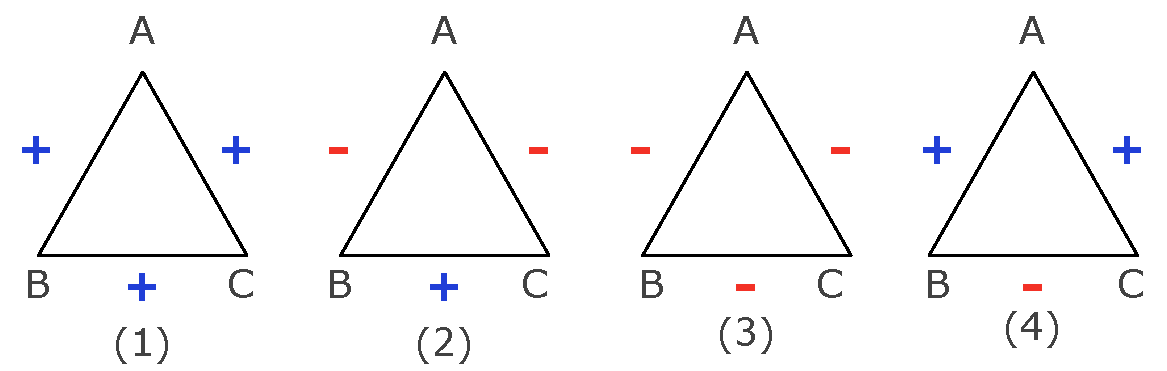
\includegraphics[height=0.8in]{Figs/strongBalance_ver.pdf}
\vspace*{-0.1in}
\caption{\label{fig:balance_strong} Classic structural balance with four different types of triads}
\end{figure}

Structural balance theory (SBT) is based on the assumption that
certain types of relationships when viewed from a local perspective
are more natural for psychological reasons~\cite{kleinberg-book}. The
local level is defined as a triangle or triad consisting of
relationships between three people.  It is natural for three people to
be friends: Alice (A) is friends with Bob (B), Bob is friends with
Chris (C) and Chris is friends with Alice. This triangle (marked (1)
in Figure~\ref{fig:balance_strong}) is considered completely
positive. Similarly, a relation where two friends, Alice and Bob have
a common enemy Chris, is also natural (triangle (2) in
Figure~\ref{fig:balance_strong}). It is considered that in such
natural relationships, there is no tension in the
interactions. However, it is less natural for Alice and Bob, and Bob
and Chris to be friends, but Alice and Chris to be enemies (triangle
(4) in Figure~\ref{fig:balance_strong}). This situation is likely to
generate tension as now Alice must avoid spending time with Bob when
Chris is around. As a result, all definitions of structural balance
would consider triangles 1 and 2 as balanced, and 4 as imbalanced.

The last type of relationship is one containing all negative
edges. This type of relationship can be considered balanced as there
is no specific conflict when three people all dislike each other but
spend no time together. As a result, in Davis's weak structural balance theory
(WSBT), triangle (3) is considered balanced~\cite{kleinberg-book}\cite{Davis:67}.  However, there is an
opportunity for one of the pairs in this triangle to become friends,
and team up against the common enemy. For this reason, (strong) SBT,
considers triangle (3) unbalanced as well~\cite{Cartwright:56}\cite{kleinberg-book}.

A complete network in which all pairs of people are connected to each
other satisfies the WSBT if all triangles in it are balanced with
respect to WSBT. In this case, the network can be divided into a set
of communities $C_1,\ldots, C_k$ such that within each community,
nodes are positively connected, and across different communities, all
connections are negative. This main result underlies many trust
inference algorithms. Algorithms that attempt to solve the {\it edge
  sign prediction problem} which involves assessing which links in a
network are positive and which links are negative, are often based on
SBT/WSBT either implicitly or explicitly.

%%  develop methods to assess
%% which nodes are likely to be connected by positive
%% edges~\cite{DuBois:2009} and which sets of nodes are
%% likely to be connected by negative edges~\cite{Leskovec:2010}. 

Guha et. al.~\cite{Guha:04} introduce one of the earliest methods that
addresses the propagation of both trust and distrust. They propose the
concepts of direct propagation, co-citation and backwards propagation,
and compute trust propagation by repeating matrix operations that
combine the three types of propagations. They report an overall $85\%$
prediction accuracy over data samples from Epinion that has equal
number of positive and negative edges.  Leskovec, Huttenlocher and
Kleinberg~\cite{Leskovec:2010} conduct a series of experiments on
three large datasets: Epinions, Slashdot and Wikipedia. In particular,
they collect two classes of features, one of which is based on degree
and the other is based on triads. These relatively local features form
a high dimensional space on which they perform standard machine
learning methods and perform edge sign predictions. Similar to our
work, they interpret some of their results in terms of the classical
balance theory~\cite{Cartwright:56}, but unlike our work, they do not
use balance theory as a starting point.

The recent work by DuBois et. al.~\cite{golbeck:distrust2011} is also
related to our paper from an algorithmic point of view. This work
stands out as it provides very good prediction performance for the
edge sign prediction problem; $80-90 \%$ on all of the three datasets
used in~\cite{Leskovec:2010} for both positive and negative edges. In this work, two
features are computed for each signed edge: the first one is based on path
probability (PP, $O(n^2)$)~\cite{DuBois:2009} and the second one uses
a force directed algorithm (FD, $O(kn)$ at each iteration where $k$ is
the average degree of the network)~\cite{golbeck:distrust2011}. In
the method of FD, the authors map trust and distrust relationships to metric
distances: the larger the distance is, the more negative (less
positive) the relation is. Then, the edge sign prediction problem is
mapped to a graph drawing problem. In this paper, we show that some of the assumptions underlying this
algorithm can be formally defined as part of a general structural
balance theory that not only works for simple positive and negative
edges, but also takes into account trust strength when
applicable. Being able to deal with strength also enables us to state
the explicit optimization criteria in the metric space for the graph
drawing problem. As a result, we are able to compare the prediction
performance with respect to an optimal placement of nodes according to
our theory. We show our method matches and outperforms the results of
this method for different data sets.

Notice that both the force directed algorithm (FD)
from~\cite{golbeck:distrust2011} and the stress majorization (SM) that
we use in this paper have been used in the field of graph
drawing~\cite{Gansner:05}. In FD, an attractive force is assigned
between endpoints of each positive edge and a repelling force is
assigned between endpoints of each negative edge. Nodes are initially
randomly laid out, and the system is simulated until a stable
equilibrium is reached when the total kinetic energy is below certain
threshold. The relation between every pair of nodes is represented by
the distance between the two end nodes in the stable layout of the
network.

While FD is simple to implement, it operates on a local pairwise
level, instead of a global level. This can lead to problems if the
local forces end up not being sufficient to hold small groups
together. Alternatively, if negative forces are too high, then the
network may continuously expand in space and the algorithm may never
converge. As a result, FD requires carefully tuned
parameters for a specific network.  In contrast, SM is a
mature approach that guarantees monotonic convergence for drawing
graphs. Moreover, in~\cite{golbeck:distrust2011}, there is no force
between pairs of unconnected nodes which can result in unintuitive
distances for such pairs. In fact as we show in our results, the FD
method maps unconnected nodes to a predominantly positive range. This
presents a problem for using this algorithm for solving the
{\it link prediction problem}~\cite{Kleinberg:03}. Link prediction is
a harder problem since networks are often sparse and one needs to find
the few edges that are true positive with high
probability. We show that our results are very promising on this
front.

In addition, to the best of our knowledge, none the existing methods
provide a principled way to study the principles underlying trust and
distrust relationships in very large networks with varying degrees of
relationship strengths. It is unclear to which degree SBT or WSBT
balance theory is valid for many large networks in which some or most
relationships are simple acquaintances~\cite{Granovetter:1973} instead
close friendship relationships. An acquaintance may not result in the
same type of structural constraints. For example, if Alice knows Bob,
and Bob knows Chris, but Chris dislikes Alice, this may not cause
much stress in the existing relationships if Alice, Bob and Chris
rarely spend time with each other, i.e. their relationship is not
strong. However, there are still some implications for the network
overall when we consider acquaintances as well as friendships. We
examine those in the next sections and provide a flexible theory of
balance that generalizes WSBT. We show that our theory allows us to
formulate convergence as an optimization problem, which can be solved
by stress majorization and illustrate that our algorithm achieves
better performance than those cited in the
literature~\cite{golbeck:distrust2011} while also providing a
principled way to approach the link prediction problem when signed
edges are present.

%%  Finally, when links are not present between
%% nodes in a network, there are multiple interpretations. It could be
%% that some nodes do not know each other or we do not know the actual
%% relationship in these cases. In both cases, we can use an inference
%% algorithm to find such edges. However, an alternate explanation could
%% be that the trust relationship is neutral, it has not yet reached a
%% point that it would be considered positive or negative. The
%% distinction in this case is that a neutral relation can become
%% positive or negative, knowing this 
